%!TEX root = ../talk.tex

\section{Python}\label{sec:python}

%%%
\subsection{A short introduction on Python}
%%%

\begin{frame}
  \MyLogo
  \frametitle{Python: A general-purpose programming language}  

\small 

\begin{itemize}

\item Created by Guido van Rossum in 1989 and first released in 1991

\item Named after ``the Monty Python'' (British comedy group)

\item An interpreted language---simple, clear, and readable 

\item Python has many excellent packages for machine learning

\item The language of choice in introductory programming courses

\end{itemize}

\begin{figure}[htbp] %  figure placement: here, top, bottom, or page
   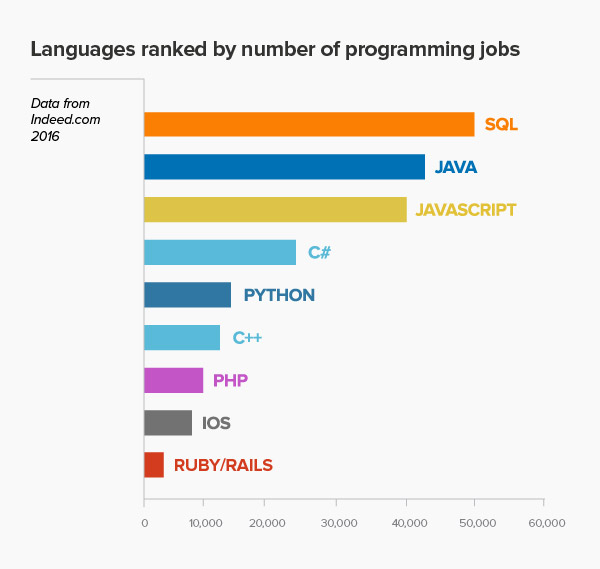
\includegraphics[height=1.7in]{figures/ComputerLanguagesDemand.jpg} 
   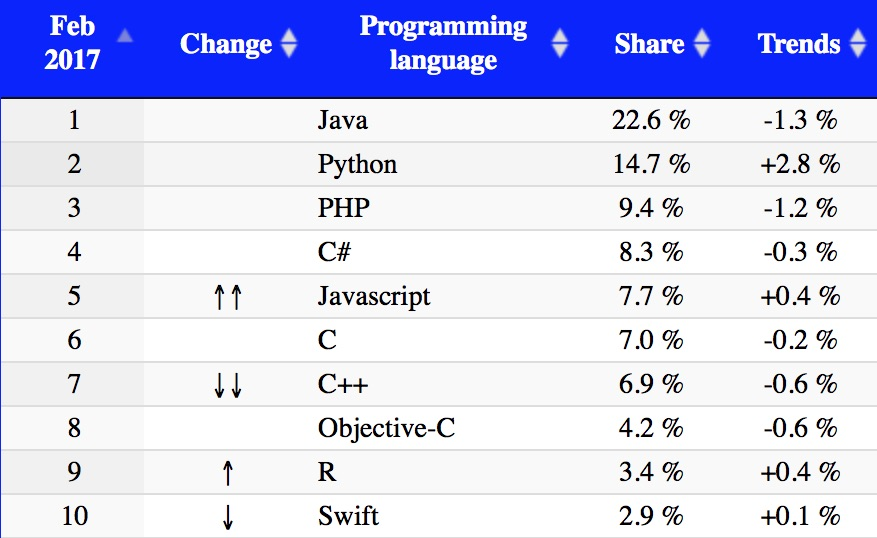
\includegraphics[height=1.7in]{figures/ComputerLanguagesShare.jpg} 
\end{figure}

\end{frame}

%%%

\begin{frame}
  \MyLogo
  \frametitle{Python for Scientific Computing}  

\small

\structure{Why Python for scientific computing?}
\begin{itemize}
	\item Strong introspection capabilities (???What does even mean???)
	\item Full modularity, supporting hierarchical packages
	\item Exception-based error handling
	\item Dynamic data types and automatic memory management
\end{itemize}

\structure{Why consider such a slow language for simulation?}
\begin{itemize}
	\item Good for proof-of-concept
	\item Implementation time versus execution time
	\item Code readability and maintenance --- short code, fewer bugs
	\item Well-written Python code is ``fast enough'' for most computational tasks
	\item Time critical parts executed through compiled language or \alert{available packages}
\end{itemize}

\end{frame}

%%%
\subsection{Basic language components}
%%%

\begin{frame}
  \MyLogo
  \frametitle{Built-in Data Structures}  
\small

\begin{itemize}
	\item Numeric types--int, float, complex, ex: a=1, b=1.0, c=1L, d=0xf, e=010, f=1+2j
	\item Sequence types--list, tuple, str, dict, ex: g=[3.14, True, 'Yes', [1], (1L,)] + [False] + [None]*3, h=(3.14, True, 'Yes', [1], ()), i='Hello' + "," + '''world!''', j=\{1: 'int', 'pi': 3.14\}

\end{itemize}

\end{frame}

%%%

\begin{frame}
  \MyLogo
  \frametitle{Control Flow}  
\small

\begin{itemize}
	\item If-then-else
	\item For loop
	\item While loop
\end{itemize}

\end{frame}

%%%

\begin{frame}
  \MyLogo
  \frametitle{Functions and Modules}  
\small

\begin{itemize}
	\item Defining functions
	\item Using modules
\end{itemize}

\end{frame}
